\section{Words and programming our problem}

\subsection{How to code a tree ? }

A computer has no natural way to see what is a tree.

One way to see a Shroeder tree with $n$ leaves is to consider them as a initial chain in the poset $\IP{n}$ using the decomposition given at example~\ref{Eg:tree_left}. This decomposition is made such that one should make the merging of all the left blocks before merging any block on the left side.

\begin{Rq}
	In other words, we are reading the tree from left to right.
\end{Rq}
\begin{Eg} The decomposition of the tree
	\raisebox{-0.5\height}{\begin{tikzpicture}[line cap=round,line join=round,>=triangle 45,x=0.2cm,y=0.2cm]
			\draw (0,0)--(0,5);
			\draw (0,1)--(-4,5);
			\draw (-2.5,3.5)--(-1,5);
			\draw (-2,4)--(-3,5);
			\draw (0,1)--(4,5);
			\draw (2.5,3.5)--(2.5,5);
			\draw (2.5,3.5)--(1,5);
			\draw (1.5,4.5) -- (2,5);
	\end{tikzpicture}} is:
\begin{equation*}
	1~2~3~4~5~6~7~8, 1~(2~3)~4~5~6~7~8,(1~2~3)~4~5~6~7~8,(1~2~3)~4~(5~6)~7~8,(1~2~3)~4~(5~6~7~8),(1~2~3~4~5~6~7~8). 
\end{equation*}
\end{Eg}

Any such code of length $n$ can be interpreted, as a sequence of $0,1$ of length $n-1$ with the bijection:
\[
\varphi: \left\lbrace\begin{array}{rcl}
	\IP{n} & \rightarrow & \{0,1\}^{n-1} \\
	P & \mapsto & (\varphi(P)_i)_{i\in\IEM{1}{n-1}}
\end{array} \right.
\]
such that for any $i\in\IEM{1}{n-1}$:
\[
\varphi(P)_i=\begin{cases}
	1 &\text{ if } i \text{ and }i+1 \text{ are un the same block in }P, \\
	0 & \text{else}.
\end{cases}
\]

\begin{Not}
	For any $n\in\N,P\in\IP{n}$, we will denote $p$ the image of $P$ by $\varphi$.
\end{Not}

Let us introduce the \emph{Hamming weight} for binary words:
\begin{defi}[Hamming weight]
	Let $W=W_1\dots W_k$ be a finite word over the alphabet $\{0,1\}$, we define its \emph{Hamming weight} as:
	\[
	\omega(W)=\left|\{ i\in\IEM{1}{k} \,|\, W_i=1\}\right|.
	\]
\end{defi}
\begin{Eg}
	For instance:
	\[
	\omega(0011011)=4.
	\]
	the word $0011011$ encodes the partition $1~2~(3~4~5)~(6~7~8)\in\IP{8}.$
\end{Eg}

Now, we can identify any initial chain, as a sequence of words of $\{0,1\}$. 
\begin{Eg}\label{Eg:tree_code}
	For instance:
	\begin{align*}
		\raisebox{-0.5\height}{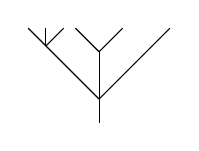
\begin{tikzpicture}[x=0.3cm, y=0.3cm]
			\draw (0,0)--(0,1);
			\draw (0,1)--(-3,4);
			\draw (0,1)--(3,4);
			\draw (0,1)--(0,3);
			\draw (0,3)--(-1,4);
			\draw (0,3)--(1,4);
			\draw (-2.25,3.25)--(-2.25,4);
			\draw (-2.25,3.25)--(-1.5,4);
		\end{tikzpicture}} && \rightarrow && \begin{array}{c}
		1~2~3~4~5~6 \\
		(1~2~3)~4~5~6 \\
		(1~2~3)~(4~5)~6 \\
		(1~2~3)~(4~5~6) \\
		(1~2~3~4~5~6)
		\end{array}
		 && \rightarrow &&  \begin{array}{ccccc}
		0 & 0 & 0 & 0 & 0 \\
		1 & 1 & 0 & 0 & 0 \\
		1 & 1 & 0 & 1 & 0 \\
		1 & 1 & 1 & 1 & 1
	\end{array} && \rightarrow && \begin{array}{c}
	0 \\ 3 \\ 11 \\ 15
	\end{array}
	\end{align*}
\end{Eg}

In the following, we will delete the beginning and the ending of such chains. Moreover, reading the chains as a sequence of words over $\{0,1\}$ one has:
\begin{Prop}\label{prop:words_chains_correspondence}
	Consider $(P_0,P_1,\dots, P_{k-1},P_k)$ an initial chain in the poset $\IP{n}$. Hence, $(p_0,p_1,\dots,p_{k-1},p_k)$ is an increasing sequence for the Hamming weight and for any $i\in\IEM{1}{k-1}$:
	\[
	\begin{cases}
		\omega(p_0)&=0, \\
		\omega(p_k)&=n-1, \\
		p_i \land p_{i+1}&=p_i, \\
		p_i \lor p_{i+1}&=p_{i+1}.
	\end{cases}
	\]
\end{Prop}
\begin{Rq}
	We know each Schroeder tree $t$ with $n$ leaves can be seen as an initial chain in the poset $\IP{n}$. Denoting this chain by $(P_0,\dots,P_k)$, we will call $(p_0,\dots,p_k)$ the \emph{code} of the tree $t$.
	In example
\end{Rq}
%Ce doit être une bijection entre les deux.

We then adapt the definition~\ref{defi:products of chains} to chains of proposition~\ref{prop:words_chains_correspondence}:
\begin{defi}
		Let $n,m\in\Nz$ and consider $S$ an increasing sequence for Hamming weight of length $n$ and $D$ another such sequence of length $m$.
		We define the following associative law:
	\begin{equation*}
		S\circ D=\left( S_1\cdot D_1,S_2\cdot D_1,\dots, S_k\cdot D_1,S_k\cdot D_2,\dots,S_k\cdot D_l\right).
	\end{equation*}
\end{defi}
\begin{Rq}
	Note that the sequences defined in proposition~\ref{prop:words_chains_correspondence} is closed under $\circ$.
\end{Rq}

Now, we need to make a bridge between the description of the operations $\prec,\cdot$ and $\succ$ from the point of view of trees to the point of view of chains defined in proposition~\ref{prop:words_chains_correspondence}.

\subsection{How to describe the $\prec, \succ$ and $\cdot$ operations ?}

In this subsection, for sake of simplicity we will not consider shuffles (respectively quasi-shuffles) but element of a symmetric group (respectively maps a packed word with at most two repetitions of one letter). 
Note that definition~\ref{def:quasiaction} extends naturally to such objects.

\subsubsection{Some clues on one example}

For instance, consider the following element of $S_7$:
\[
\sigma=(1~2~5~3~6~7~4)
\]
and consider two trees having the respective comb representations:
\begin{align*}
	s=\raisebox{-0.5\height}{\begin{tikzpicture}[line cap=round,line join=round,>=triangle 45,x=0.25cm,y=0.25cm]
		% Etage 1
		\draw (0,0)--(0,1);
		%Etage 2
		\draw (0,1)--(-1,2) node[left]{$F_{1}$};
		% Etage 3
		\draw (0,1)--(7,8);
		\draw (2,3)--(1,4) node[left]{$F_{2}$};
		%Etage 4
		\draw (4.,5.)--(3,6) node[left]{$F_3$};
		%Etage 4
		\draw (6,7)--(5,8) node[left]{$F_{4}$};
\end{tikzpicture} }, 
&& t=\raisebox{-0.5\height}{\begin{tikzpicture}[line cap=round,line join=round,>=triangle 45,x=0.25cm,y=0.25cm]
% Etage 1
\draw (0,0)--(0,1);
%Etage 2
\draw (0,1)--(1,2) node[right]{$F_{1}$};
% Etage 3
\draw (0,1)--(-5,6);
\draw (-2,3)--(-1,4) node[right]{$F_{2}$};
%Etage 4
\draw (-4,5)--(-3,6) node[right]{$F_{3}$};
\end{tikzpicture}}.
\end{align*}
Hence:
\[
\sigma(t,s)=\raisebox{-0.5\height}{
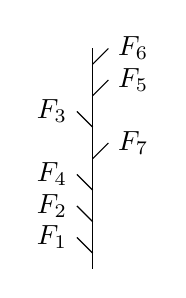
\begin{tikzpicture}[x=0.2cm, y=0.2cm]
	\draw (0,0)--(0,14);
	\draw (0,1)--(-1,2);
	\draw (0,3)--(-1,4);
	\draw (0,5)--(-1,6);
	\draw (0,7)--(1,8);
	\draw (0,9)--(-1,10);
	\draw (0,11)--(1,12);
	\draw (0,13)--(1,14);
	% décors des forêts
	\draw (-1,2) node[left] {$F_1$};
	\draw (-1,4) node[left] {$F_2$};
	\draw (-1,6) node[left] {$F_4$};
	\draw (1,8) node[right] {$F_7$};
	\draw (-1,10) node[left] {$F_3$};
	\draw (1,12) node[right] {$F_5$};
	\draw (1,14) node[right] {$F_6$};
\end{tikzpicture}
}
\]

Can we interpret this action with the words over $\{0,1\}$ encoding the tree ? 


Take a simpler example:
\[
	t=	\raisebox{-0.3\height}{\begin{tikzpicture}[line cap=round,line join=round,>=triangle 45,x=0.3cm,y=0.3cm]
		% Etage 1
		\draw (0,0)--(0,1);
		%Etage 2
		\draw (0,1)--(-1,2) node[left]{$F_1$};
		% Etage 3
		\draw (0,1)--(2,3);
		\draw (1,2)--(0,3);
		\draw (0,3.5) node[left]{$F_2$};
\end{tikzpicture}} \text{ and } s= \raisebox{-0.3\height}{\begin{tikzpicture}[line cap=round,line join=round,>=triangle 45,x=0.3cm,y=0.3cm]
		% Etage 1
		\draw (0,0)--(0,1);
		\draw (0,1) --(-1,2);
		%Etage 2
		\draw (0,1)--(1,2) node[right]{$F_{3}$};
\end{tikzpicture}}.
\]
with $F_1=\Y, F_2=\balais$ and $F_3=||$.
Consider $\sigma=(1~3~2)$, then:
\[
\sigma(t,s)=\raisebox{-0.5\height}{
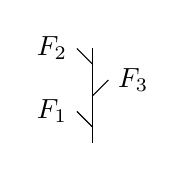
\begin{tikzpicture}[x=0.2cm,y=0.2cm]
	\draw (0,0)--(0,6);
	\draw (0,1)--(-1,2) node[left] {$F_1$};
	\draw (0,3)--(1,4) node[right] {$F_3$};
	\draw (0,5)--(-1,6) node[left] {$F_2$};
\end{tikzpicture}}=\raisebox{-0.5\height}{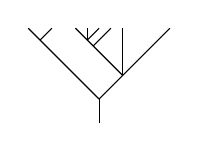
\begin{tikzpicture}[x=0.3cm, y=0.3cm]
\draw (0,0)--(0,1);
%partie gauche
\draw (-2.5,3.5)--(-2,4);
\draw (0,1)--(-3,4);
%partie droite
\draw (0,1)--(3,4);
\draw (1,2)--(-1,4);
\draw (1,2)--(1,4);

\draw (-0.5,3.5)--(0,4);
\draw (-0.5,3.5)--(-0.5,4);
\draw (-0.25,3.25)--(0.5,4);
\end{tikzpicture}}.
\]
With this simpler example, we notice $t$ has $6$ leaves and $s$ has $3$ leaves. So $\sigma(t,s)$ has $8$ leaves.

Now, let us look at the code of these two trees:
\begin{align*}
	t=\begin{array}{cccccc}
		0 & 0 & 0 & 0 & 0  \\
		1 & 0 & 0 & 0 & 0 \\
		1 & 0 & 1 & 1 & 0 \\
		1 & 0 & 1 & 1 & 0
	\end{array} \text{ et } s=
	\begin{array}{cc}
		0 & 0 \\
		1 & 1
	\end{array}
\end{align*}
The "code" of $\sigma(t,s)$ is:
\begin{equation};\label{Eq: example_tridend_code}
	\begin{NiceArray}{|ccccccc}[first-col]
		& 0 & 0 & 0 & 0 & 0 & 0 & 0  \\
		F_1		  & 1 & 0 & 0 & 0 & 0 & 0 & 0  \\
		F_2		  & 1 & 0 & 1 & 1 & 0 & 0 & 0  \\
		F_2\cdot g& 1 & 0 & 1 & 1 & 1 & 0 & 0  \\
		F_3		  & 1 & 0 & 1 & 1 & 1 & 1 & 1  \\
		F_3\cdot g^2& 1 & 1 & 1 & 1 & 1 & 1 & 1 \\
		g\cdot F_1& 1 & 1 & 1 & 1 & 1 & 1 & 1
	\end{NiceArray}.
\end{equation}
In equation~\ref{Eq: example_tridend_code}, this is not the real code because one should delete the line indexed with $F_3$. But it shows how to build from a quasi-shuffle 
the code of this tree with the labels. Actually, when one sees a $F_i$ on the left hand side of the table in equation~\ref{Eq: example_tridend_code}, one should copy the code of $F_i$ at the indices of the leaves in $F_i$ in the shuffled tree, and when one sees a $F_i\cdot g^j$ where $j$ is the number of forests in $F_i$ (respectively $g^j \cdot F_i$) it replaces $j$ zeros reading from right to left (respectively from left to right) beginning with the rightmost (respectively leftmost) zero touching the code of $F_i$.

More rigorously, let us define:
\begin{defi}[forest code]
	Let $F$ be a forest $F=t_1\cdot \dots \cdot t_k$. For any $i\in\IEM{1}{k}$, put $C_i$ the code of the tree $t_i$. The \emph{forest code} of $F$ is:
	\[
	C_1\circ 0 \circ C_2 \circ 0 \circ \dots \circ 0 \circ C_k.
	\]
\end{defi}

\begin{Not}
	We put $C_|$ the code given by $0$.
\end{Not}
\begin{Eg}
	Let $F=\Y~\balais~|$, its code $C$ is:
	\[
	\begin{array}{cccccc}
		0 & 0 & 0 & 0 & 0 \\
		1 & 0 & 0 & 0 & 0 \\
		1 & 0 & 1 & 1 & 0 \\
	\end{array}
	\]
\end{Eg}
\begin{Rq}
	The code of $|$ is restrained to $0$, hence  the result of $C\circ C_|$ is simply the concatenation of a zero to every word in the code $C$.
\end{Rq}

\begin{Not}
	Denote $C_i$ the code of any forest $F_i$ for $i\in\IEM{1}{n}.$
\end{Not}

We introduce a family of operators on the set of forests codes:
\begin{defi}[Left and right closure operator]
	Let $S$ be a sequence of $0$ and $1$ with $j$ zeros. Let us denote:
	\[
	S=0^{n_0}~1^{m_1}~0^{n_1}~\dots~0^{n_{l-1}}~1^{m_l}~0^{n_l}.
	\] Let $k\in\IEM{1}{j}$. 
	We define the \emph{right} (respectively left) \emph{closure operator of order} $k$ over the set of code with rightmost (respectively leftmost) element equal to $0$. We denote it by $\leftarrow g^k$ (respectively $g^k \rightarrow $). The image of the sequence $S$ is the same sequence where we have replaced the $k$ firsts zeros by ones reading from right to left (respectively from left to right). 
\end{defi}
\begin{Egs}For instance:
	\begin{align*}
		0 ~ 1 ~ 1 ~ 0 ~ 1 ~ 0 ~ 0 ~ 0 \leftarrow g^3&= 0 ~ 1 ~ 1 ~ 0 ~ 1 ~ 1 ~ 1 ~ 1, \\
		g^3 \rightarrow 0 ~ 1 ~ 1 ~ 0 ~ 1 ~ 0 ~ 0 ~ 0 &= 1 ~ 1 ~ 1 ~ 1 ~ 1 ~ 1 ~ 0 ~ 0.
	\end{align*}
\end{Egs}

\begin{Not}
	We denote $\mathcal{C}$ the set of forests code. Moreover, we define:
	\begin{enumerate}
		\item $\mathcal{C}_0$ the subset of $\mathcal{C}$ such that the forests code ends with $0$;
		\item $_0\mathcal{C}$ the subset of $\mathcal{C}$ such that the forests code begins with $0$;
	\end{enumerate}
\end{Not}

\begin{defi}
	Let $C$ be a forest code. We define two following maps:
	\begin{align*}
		L_0:\left\lbrace\begin{array}{rcl}
			\mathcal{C} & \rightarrow & \mathcal{C}_0 \\
			C & \mapsto & C\circ C_| ,
		\end{array}\right. && {_0L}:\left\lbrace\begin{array}{rcl}
			\mathcal{C} & \rightarrow & {_0\mathcal{C}} \\
			C & \mapsto & C_|\circ C. 
		\end{array}\right.
	\end{align*}
\end{defi}
\begin{Rq}
	For trees, this operation is just the right or left concatenation of $|$.
\end{Rq}

Let us introduce:
\begin{defi}[The forest code grafting operator]
	Let $C$ and $D$ be two forest code and let $n$ and $m$ be the number of zeros in $C$ and $D$. Put $F$ and $G$ the forests associated respectively to $C$ and $D$.  We define the maps $f_r:\mathcal{C}_0\times\mathcal{C}\rightarrow \mathcal{C}$ and $f_l:{_0\mathcal{C}}\times \mathcal{C}\rightarrow \mathcal{C}$ defined by:
	\begin{align*}
		f_r(D,C)&=(C\circ D)\leftarrow g^{n+m}, \\
		f_l(D,C)&=g^{n+m} \rightarrow (D\circ C).
	\end{align*}
	The trees corresponding to those codes are:
\end{defi}
\begin{Eg}
	Consider $F$ a forest and its forest code $C$. Then, $f_r(C_|,C)$ and $f_l(C_|,C)$ are respectively encoding the following trees:
	\[
	\labY{F}{} \text{ and } \labY{}{F}.
	\]
\end{Eg}
\begin{Lemme}
	Let $F$ and $G$ be two forests with respective code $C_F$ and $C_G$. Then, the codes below correspond to the trees:
	\begin{align*}
		f_l(L_0(C_G),C_F) \rightarrow \labY{G}{F}, &&
		f_r({_0L}(C_G),C_F) \rightarrow \labY{F}{G}. 
	\end{align*}
\end{Lemme}
\begin{proof}
	Easy.
\end{proof}
\begin{Rq}
	The number of zeros in a forest code is exactly the number of trees in the forest associated to it.
\end{Rq}

Consider two trees with the following combs representations:
\begin{align*}
	t=\peignedroit{1}{2}{k} && \text{ and } &&  s=\peignegauche{k+1}{k+2}{k+l},
\end{align*}

Let us denote for any $i\in\IEM{1}{k+l},C_i$ the forest code of $F_i$ and $n_i$ the number of forests of $C_i$. Put $C_t$ the code of $t$ and $C_s$ the code of $s$. Hence, their respective code are (with polish notations):
\begin{align*}
	C_t&=f_r\underbrace{L_0f_r\dots L_0f_r}_{(k-1) \text{ times}}C_|C_k\dots C_2 C_1, \\
	C_s&=f_l\underbrace{{_0L}f_l\dots {_0L}f_l}_{(l-1) \text{ times}}C_|C_k\dots C_2 C_1.
\end{align*}

We introduce a final notation before giving the action of quasi-shuffles over those tree codes:
\begin{Not}
	Let $C$ be a code, we denote $\len(C)$ the length of $C$.
\end{Not}

\begin{defi}
	Let $\sigma\in S_{k+l}$ and put $C_i$ the code of the forest $F_i$ for all $i\in\IEM{1}{k+l}$. Put $n=\max(\sigma)$.
	\begin{enumerate}
		\item put $\tau_1=\sigma^{-1}|_{\IEM{1}{k}}$ and begin with:
		\[
		D_0=L_0(C_{\tau_1(1)})\circ \dots \circ L_0(C_{\tau_1(k)}) .
		\]
		\item put $\tau_2=\sigma^{-1}|_{\IEM{k+1}{k+l}}$ and for all $i\in\IEM{1}{n}$ compute iteratively:
		\begin{align*}
			D_i&=\begin{cases}
				f_r(D_{i-1},C_{j'}) &\text{ if } \exists (j,j')\in\IEM{1}{k}\times\IEM{k+1}{k+l},\sigma(j')=\sigma(j)=i, \\
				D_{i-1} & \text{ if } \exists j\in\IEM{1}{k}, \sigma(j)=i \text{ and } i\notin \ima(\tau_2),\\
				f_lD_{i-1} C_{j'}  &\text{ if } \exists j'\in\IEM{k+1}{k+l}, \sigma(j')=i \text{ and } i\notin \ima(\tau_1).
			\end{cases}
		\end{align*}
		Define $D_n\coloneqq\sigma(C_t,C_s)$.
	\end{enumerate}
\end{defi} 


